% Especificaciones del tamaño de letra, tamaño de hoja, márgenes, librerias, etc.
\documentclass[12pt, letterpaper]{article}
\usepackage[english]{babel}
\usepackage[utf8]{inputenc}
\usepackage[T1]{fontenc}
\usepackage{mathrsfs}
\usepackage{amsmath}
\usepackage{graphicx}
\usepackage{subcaption}
\usepackage{hyperref}
\usepackage{url}
\usepackage{amssymb}
\usepackage{float}
\usepackage[margin=1in]{geometry}
\renewcommand{\baselinestretch}{1.5}

% Enlace Bibliografía
\usepackage{csquotes}
\usepackage[notes,backend=biber]{biblatex-chicago}
\addbibresource{referencias.bib}

% Titulo, autores, fecha.
\title{Práctica \#6: Abstracción del Sistema Dinámico}
\author{Carlos Vásquez 1155057}

% Inicio del documento
\begin{document}
\maketitle
\section*{Introducción}

Las capas de abstracción proporcionan una manera más sencilla y conveniente para lograr analizar un sistema y que no olvidemos el objetivo general de éste. Estas abstracciones se hacen a lo largo de todas las ciencias e ingenierías. Escribir código resulta muy útil debido a la capacidad de abstraer ideas y la posibilidad de manipular esas ideas en líneas de codigo, simplificando aquello que estamos analizando, o incluso automatizando procesos complicados e iterativos.

Para lograr comprender la importancia de estas abstracciones, podemos ver dos ejemplos que se utilizan arduamente en la ingeniería.

El análisis de los campos eléctrico y magnético y, por extensión, el de los circuitos eléctricos está regido por las ecuaciones de Maxwell. A pesar de ser algo complicadas éstas nos pueden ayudar a obtener información sobre las distintas características de un circuito eléctrico. Utilizar estas ecuaciones puede ser tedioso después de un tiempo, sin embargo, podemos realizar las siguientes suposiciones en un circuito eléctrico:\autocite{agarwal05}

\begin{itemize}
	\item Elegir elementos con fronteras específicas para que la razón de cambio en el flujo magnético de cualquier lazo cerrado fuera de un elemento sea cero para todo tiempo. En otras palabras, que se cumpla lo siguiente para las fronteras del elemento:
		\begin{equation}
			\frac{\partial \Phi_b}{\partial t} = 0
		\end{equation}
	\item Elegir elementos con fronteras especiales en donde no haya variación en la carga a lo largo del tiempo dentro de ese elemento. En otras palabras:
		\begin{equation}
			\frac{\partial q}{\partial t} = 0
		\end{equation}
	\item Operar en un regimen en el cual la escala de tiempo de las señales de interés sean mucho más grandes que el retraso de propagación de las ondas electromagnéticas a través de los elementos a analizar.
\end{itemize}

Al momento de analizar una situación más general, tendríamos que utilizar las ecuaciones, digamos que nos interesa saber la corriente en un cable del punto A al punto B, entonces nuestro análisis sería el siguiente:
\begin{equation}
	\int\limits_A \vec{J} \cdot dA - \int\limits_B \vec{J} \cdot dA = \frac{\partial q}{\partial t}
\end{equation}

Sim embargo, dadas las suposiciones que hemos hecho anteriormente, si nos restringimos a realizar análisis en los sistemas especificados, la ecuación 3 se simplifica a lo siguiente:

\begin{equation}
	\begin{split}
		\int\limits_A \vec{J} \cdot dA - \int\limits_B \vec{J} \cdot dA &= 0\\
		I_A - I_B &= 0
	\end{split}
\end{equation}
 Este resultado facilita el análisis de circuitos, y de manera similar ocurre con el voltaje en un circuito. De manera general realizaríamos el siguiente análisis:

 \begin{equation}
	 \varepsilon = \oint \vec{E} \cdot \vec{dl} = -\frac{\partial \Phi_B}{\partial t}
 \end{equation}

 Y si tomamos en cuenta las suposiciones anteriores y realizamos ese análisis en elementos que cumplan con ellas nuestra ecuación se reduce a:

 \begin{equation}
	 \begin{split}
		 \varepsilon = \oint \vec{E} \cdot \vec{dl} = - \frac{\partial \Phi_B}{\partial t} &= 0\\
		 \varepsilon = V_1 + V_2 + \cdots + V_n &= 0
	\end{split} 
\end{equation}

Como podemos observar en las ecuaciones 4 y 6, las leyes de voltaje y corriente de Kirchhoff (LVK y LCK) son casos particulares de las ecuaciones de Maxwell, y mientras los sistemas que analicemos cumplan estas suposiciones entonces podremos analizarlos mediante simples sumas algebráicas, dándole una capa de abstracción a nuestro análisis y volviéndolo mucho más sencillo de analizar.

Este no es el único campo que se beneficia de la abstracción, en física moderna se utilizar regularmente este tipo de simplificaciones. Física del estado sólido y física de elementos finitos se beneficia mucho de las capas de abstracción entre la realidad cruda y la idealización que realizamos sobre nuestros sistemas físicos.

\section*{Desarrollo}

Después de comprender la necesidad de realizar abstracciones para poder crear sistemas útiles y avanzados, podemos proceder con la abstracción de nuestro sistema. Anteriormente se vio nuestro sistema de la siguiente manera (ignorando las perturbaciones añadidas):

\begin{figure}[H]
	\centering
	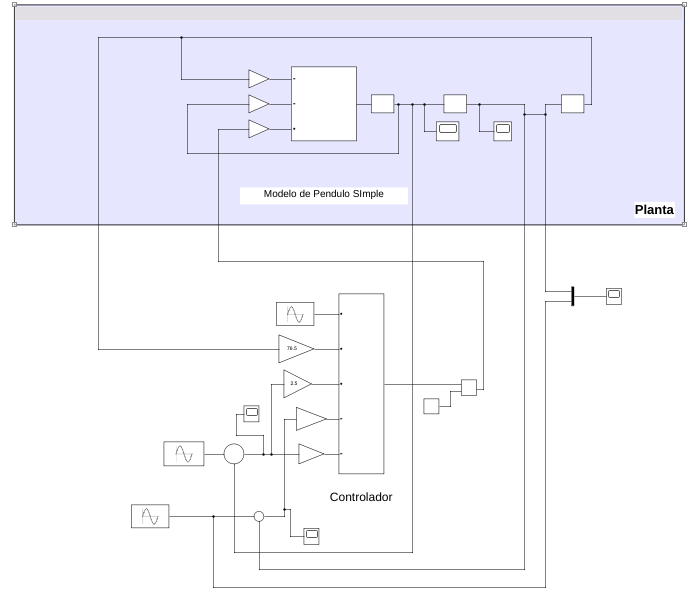
\includegraphics[width=0.7\textwidth]{system.png}
	\caption{Sistema dinámico orginial, con controlador.}
\end{figure}

El sistema lo podemos simplificar en gran medida para hacerlo visualmente más estético y fácil de comprender. Lo que se diseño fue el siguiente sistema.

\begin{figure}[H]
	\centering
	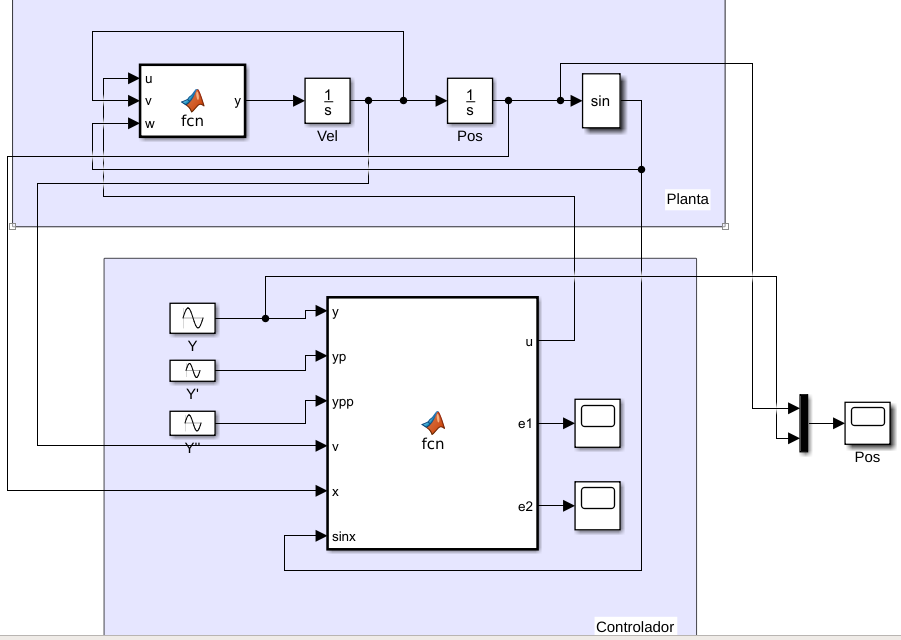
\includegraphics[width=\textwidth]{newsys.png}
	\caption{Reemplazamiento del antiguo sistema con bloques más generales.}
\end{figure}

Es de gran importancia aclarar que el sistema no ha sido modificado de manera en la que su funcionamiento sea distinto, esto simplemente nos permite visualizar qué variables están en juego en cada parte del sistema, lo cual nos hace entender más fácil el funcionamiento de éste.

Podemos ver que ahora tenemos dos bloques distintos, ambos llamados "MATLAB Function", el cual nos permite tener el número que queramos de entradas y el número que deseemos de salidas. Claro que nosotros definiremos cómo es que estas entradas interactúan entre sí y las salidas se definirán en términos de éstas. A continuación se muestra el código de los bloques de los cuales ya hemos hablado.

\begin{figure}[H]
	\centering
	\begin{subfigure}[b]{0.55\linewidth}
		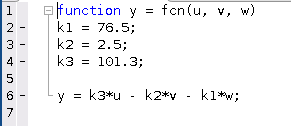
\includegraphics[width=\linewidth]{m1.png}
		\caption{Código de la función en el péndulo.}
	\end{subfigure}

	\begin{subfigure}[b]{0.75\linewidth}
		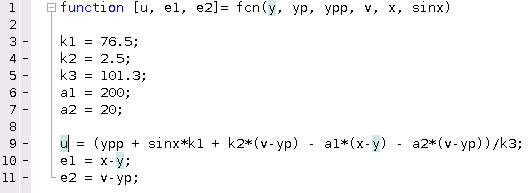
\includegraphics[width=\linewidth]{m2.png}
		\caption{Código de la función en el controlador.}
	\end{subfigure}
	\caption{Código utilizado para reemplazar el funcionamiento de los adders y gains.}
\end{figure}

Como podemos observar, hemos reducido nuestro sistema a estos bloques y manipulamos las entradas como lo hacíamos con los bloques para sumar y restar, al igual que las ganancias. El sistema anterior y este nuevo son casi identicos entre sí.

\begin{figure}[H]
	\centering
	\begin{subfigure}[b]{0.49\linewidth}
		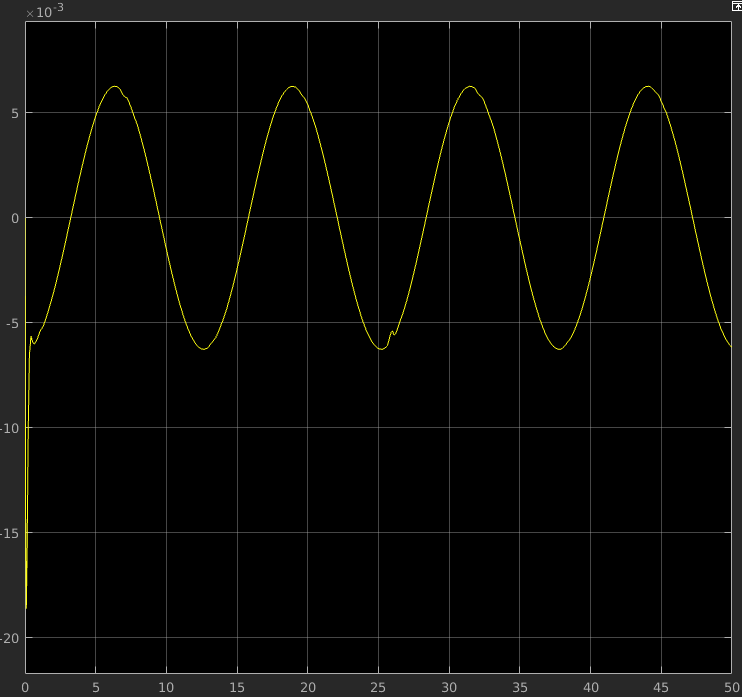
\includegraphics[width=\linewidth]{e1a200.png}
		\caption{$e_1$}
	\end{subfigure}
	\begin{subfigure}[b]{0.49\linewidth}
		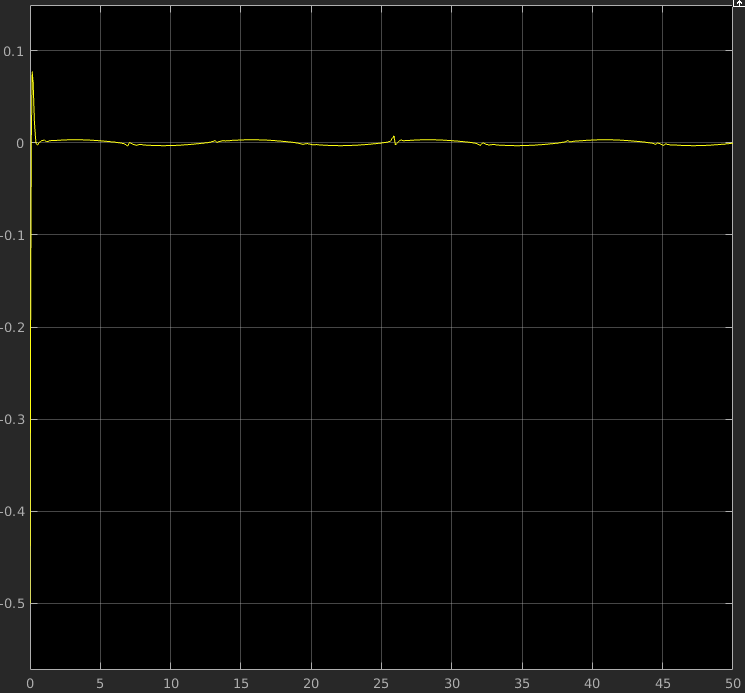
\includegraphics[width=\linewidth]{e2a200.png}
		\caption{$e_2$}
	\end{subfigure}
	\caption{Errores en el sistema original.}
\end{figure}

\begin{figure}[H]
	\centering
	\begin{subfigure}[b]{0.49\linewidth}
		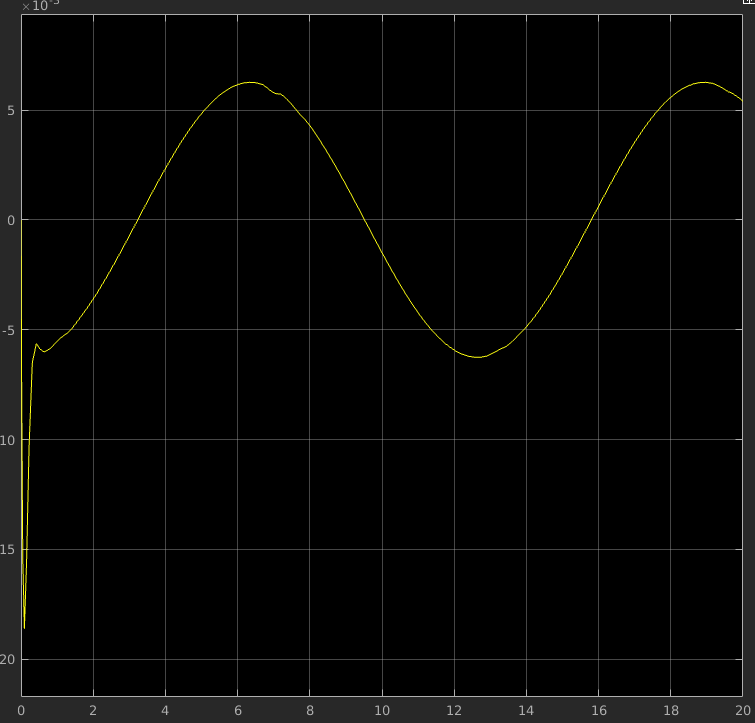
\includegraphics[width=\linewidth]{e1.png}
		\caption{$e_1$}
	\end{subfigure}
	\begin{subfigure}[b]{0.49\linewidth}
		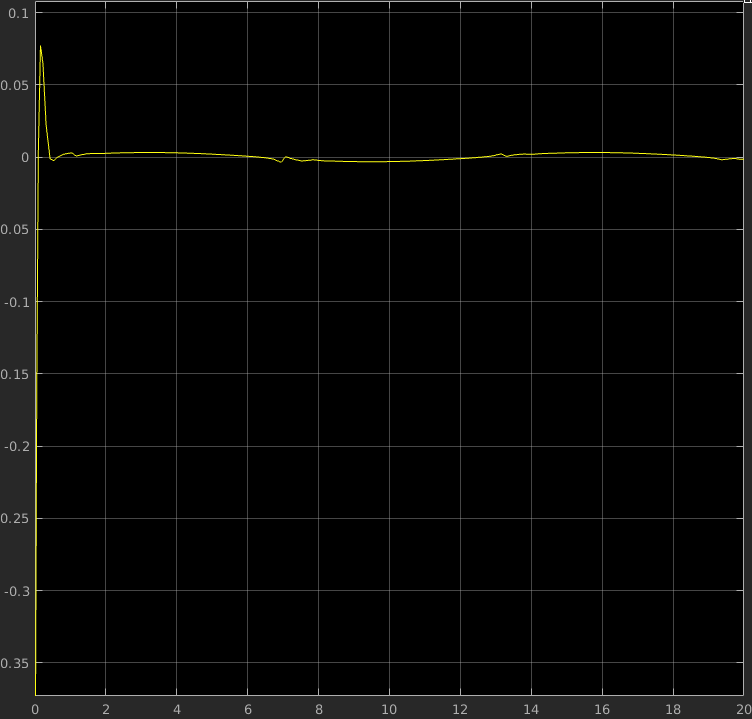
\includegraphics[width=\linewidth]{e2.png}
		\caption{$e_2$}
	\end{subfigure}
	\caption{Errores en el nuevo sistema.}
\end{figure}

\section*{Conclusión}

Como observamos en el sistema anterior, realizar esta práctica nos permite entender el sistema fácilmente, evitando los malentendidos entre las variables que se presentat. Además, así podemos visualizar de una mejor manera las variables de estado que necesita conocer nuestro controlador para poder realizar su trabajo correctamente.
%%%%%  Bib
\renewcommand\refname{Referencias}
\printbibliography
\end{document}
